\setmodule{7}

%BEGIN_FOLD % ====>>_____ Занятие 1 _____<<====
\begin{class}[number=1]
	\begin{listofex}
		\item Два ребра прямоугольного параллелепипеда, выходящие из одной вершины, равны \(1, 2\). Объем параллелепипеда равен \(6\). Найдите площадь его поверхности.
		\item Два ребра прямоугольного параллелепипеда равны \(7\) и \(4\), а объём параллелепипеда равен \(140\). Найдите площадь поверхности этого параллелепипеда.
		\item 
		\begin{minipage}[t]{\bodywidth}
			В прямоугольном параллелепипеде \(ABCDA_1B_1C_1D_1\) рёбра \(AB, BC\) и диагональ боковой грани \(BC_1\) равны соответственно \(7, \) \( 3\) и \(3\sqrt{5}\). Найдите объём параллелепипеда \(ABCDA_1B_1C_1D_1\).
		\end{minipage}
		\hspace{0.02\linewidth}
		\begin{minipage}[t]{\picwidth}
			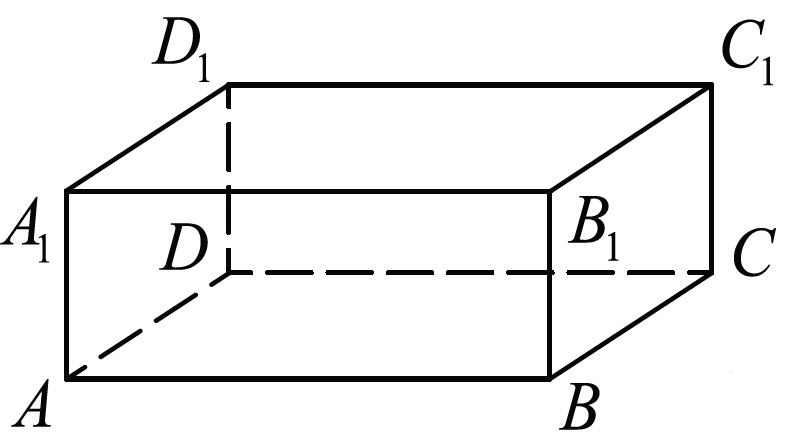
\includegraphics[align=t, width=\linewidth]{\picpath/G101M9L1-1}
		\end{minipage}
		\item 
		\begin{minipage}[t]{\bodywidth}
			В прямоугольном параллелепипеде \(ABCDA_1B_1C_1D_1\) рёбра \(CD, CB\) и диагональ \(CD_1\) боковой грани равны соответственно \(2, 4\) и \(2\sqrt{10}\). Найдите площадь поверхности параллелепипеда \(ABCDA_1B_1C_1D_1\).
		\end{minipage}
		\hspace{0.02\linewidth}
		\begin{minipage}[t]{\picwidth}
			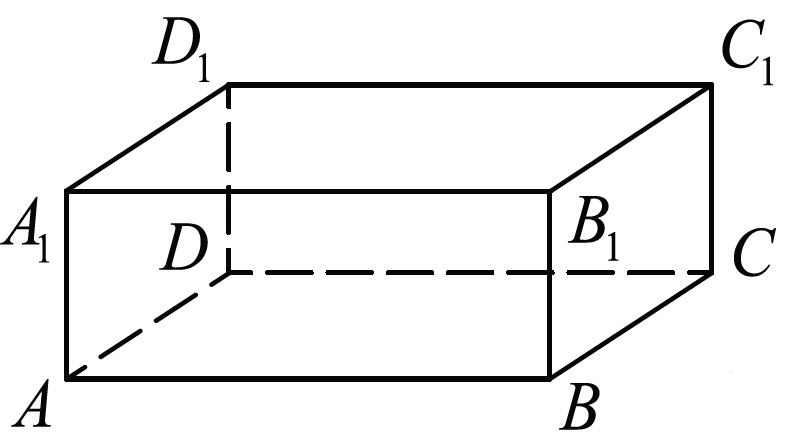
\includegraphics[align=t, width=\linewidth]{\picpath/G101M9L1-1}
		\end{minipage}
		\item Основанием прямой треугольной призмы служит прямоугольный треугольник с катетами \(6\) и \(8\), боковое ребро равно \(5\). Найдите объем призмы.
		\item В основании прямой призмы лежит прямоугольный треугольник, один из катетов которого равен \(2\), а гипотенуза равна \(\sqrt{53}\). Найдите объём призмы, если её высота равна \(3\).
		\item В основании прямой призмы лежит прямоугольный треугольник, катеты которого равны \(11\) и \(5\). Найдите объём призмы, если её высота равна \(4\).
		\item 
		\begin{minipage}[t]{\bodywidth}
			Стороны основания правильной шестиугольной пирамиды равны \(10\), боковые ребра равны \(13\). Найдите площадь боковой поверхности этой пирамиды.
		\end{minipage}
		\hspace{0.02\linewidth}
		\begin{minipage}[t]{\picwidth}
			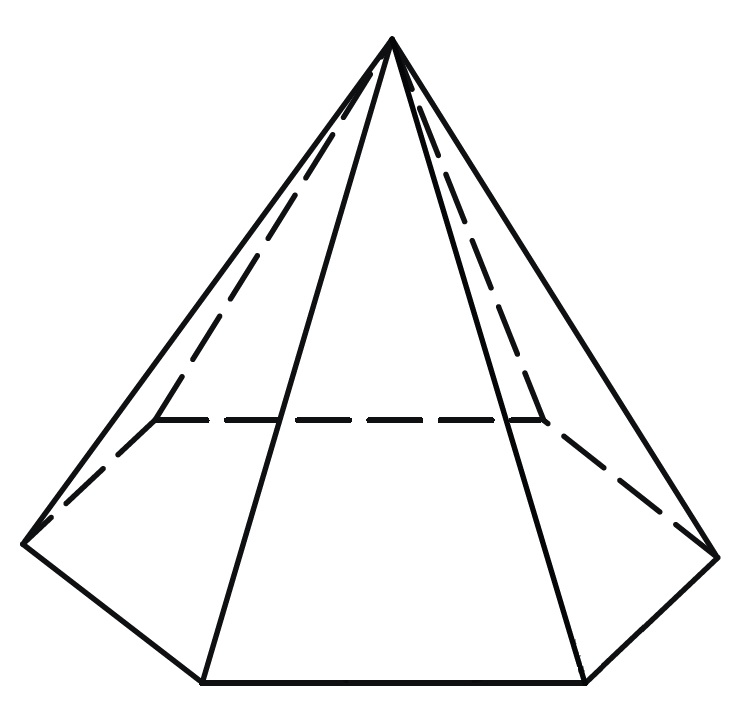
\includegraphics[align=t, width=\linewidth]{\picpath/G101M9L1-2}
		\end{minipage}
		\item 
		\begin{minipage}[t]{\bodywidth}
			Основанием пирамиды является прямоугольник со сторонами \(3\) и \(4\). Ее объем равен \(16\). Найдите высоту этой пирамиды.
		\end{minipage}
		\hspace{0.02\linewidth}
		\begin{minipage}[t]{\picwidth}
			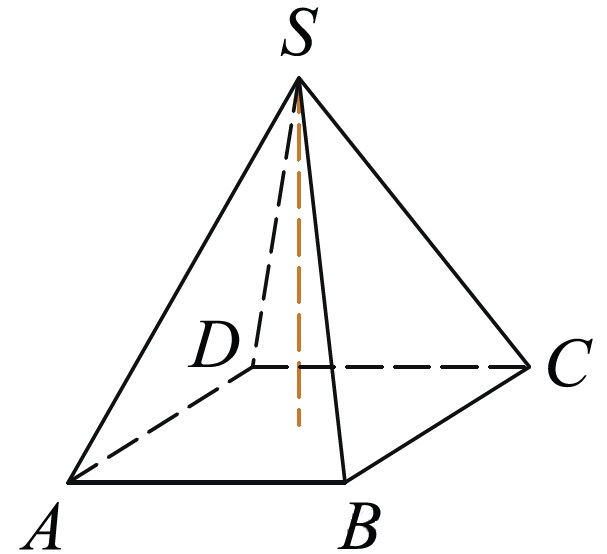
\includegraphics[align=t, width=\linewidth]{\picpath/G101M9L1-3}
		\end{minipage}
		\item 
		\begin{minipage}[t]{\bodywidth}
			Основанием пирамиды является прямоугольник со сторонами \(4\) и \(5\). Ее объем равен \(80\). Найдите высоту этой пирамиды.
		\end{minipage}
		\hspace{0.02\linewidth}
		\begin{minipage}[t]{\picwidth}
			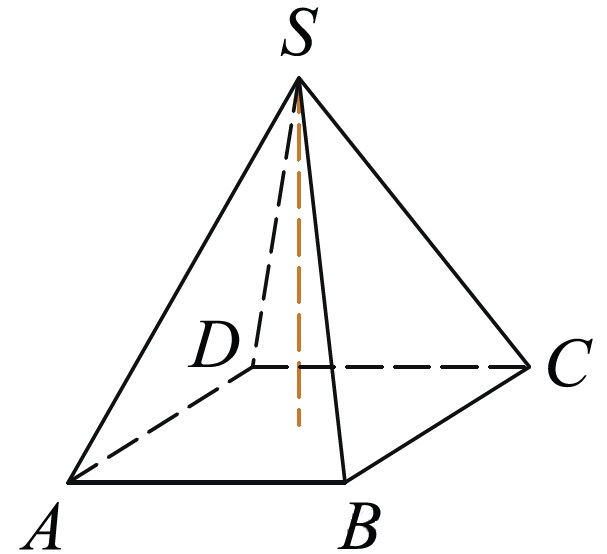
\includegraphics[align=t, width=\linewidth]{\picpath/G101M9L1-3}
		\end{minipage}
		\item 
		\begin{minipage}[t]{\bodywidth}
			Найдите объём правильной четырёхугольной пирамиды, сторона основания которой равна \(4\), а боковое ребро равно \(\sqrt{17}\).
		\end{minipage}
		\hspace{0.02\linewidth}
		\begin{minipage}[t]{\picwidth}
			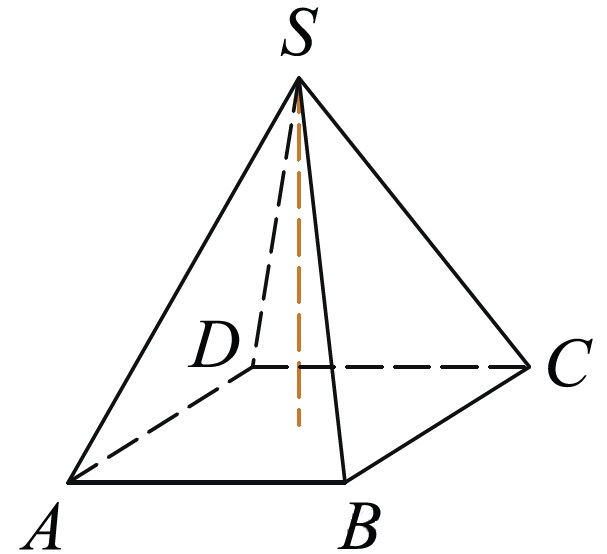
\includegraphics[align=t, width=\linewidth]{\picpath/G101M9L1-3}
		\end{minipage}
		\item 
		\begin{minipage}[t]{\bodywidth}
			В основании пирамиды \(SABC\) лежит правильный треугольник \(ABC\) со стороной \(10\), а боковое ребро \(SA\) перпендикулярно основанию и равно Найдите объём пирамиды \(SABC\).
		\end{minipage}
		\hspace{0.02\linewidth}
		\begin{minipage}[t]{\picwidth}
			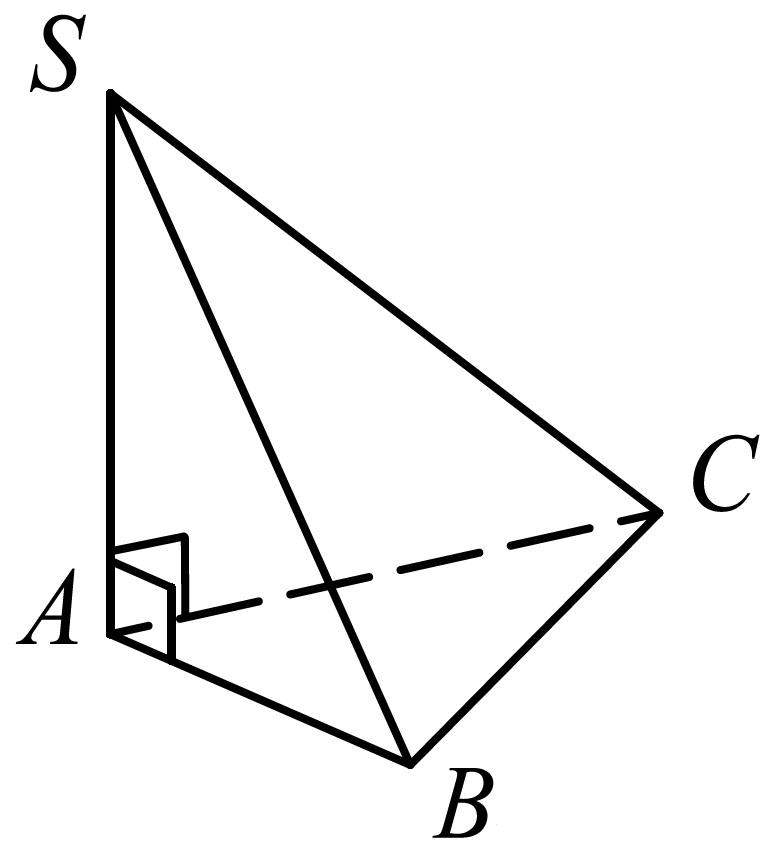
\includegraphics[align=t, width=\linewidth]{\picpath/G101M9L1-4}
		\end{minipage}
		\item 
		\begin{minipage}[t]{\bodywidth}
			В треугольной пирамиде \(ABCD\) рёбра \(AB, AC\) и \(AD\) взаимно перпендикулярны. Найдите объём этой пирамиды, если \(AB = 6, AC = 18\) и \(AD = 8\).
		\end{minipage}
		\hspace{0.02\linewidth}
		\begin{minipage}[t]{\picwidth}
			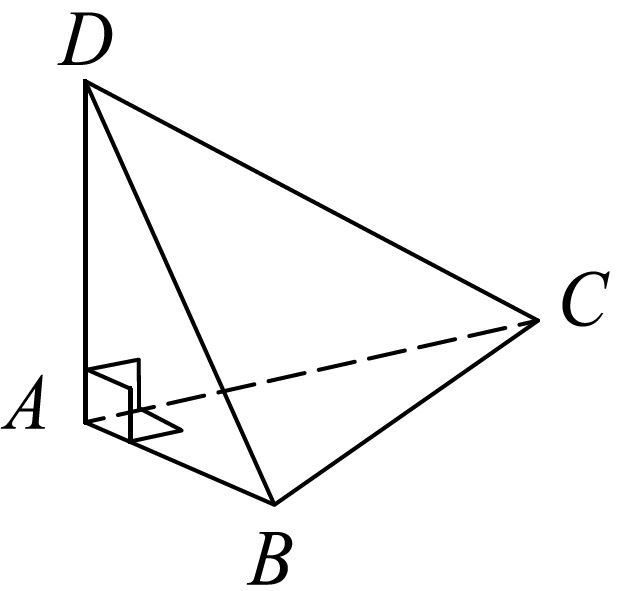
\includegraphics[align=t, width=\linewidth]{\picpath/G101M9L1-5}
		\end{minipage}
		\newpage
		\item Стороны основания правильной треугольной пирамиды равны \(16\), а боковые рёбра равны \(10\). Найдите площадь боковой поверхности пирамиды.
		\item Даны два цилиндра. Радиус основания и высота первого равны соответственно \(4\) и \(18\), а второго --- \(2\) и \(3\). Во сколько раз площадь боковой поверхности первого цилиндра больше площади боковой поверхности второго?
		
		
		%\item 
		%\begin{minipage}[t]{\bodywidth}
		%	
		%\end{minipage}
		%\hspace{0.02\linewidth}
		%\begin{minipage}[t]{\picwidth}
		%	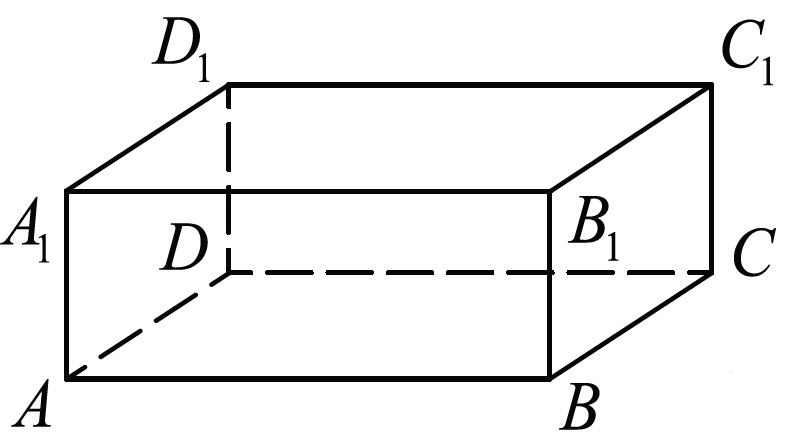
\includegraphics[align=t, width=\linewidth]{\picpath/G101M9L1-1}
		%\end{minipage}
	\end{listofex}
\end{class}
%END_FOLD

%BEGIN_FOLD % ====>>_____ Занятие 2 _____<<====
\begin{class}[number=2]
	\begin{listofex}
		\item Занятие 2
	\end{listofex}
\end{class}
%END_FOLD

%BEGIN_FOLD % ====>>_ Домашняя работа 1 _<<====
\begin{homework}[number=1]
	\begin{listofex}
		\item Домашняя работа 1
	\end{listofex}
\end{homework}
%END_FOLD

%BEGIN_FOLD % ====>>_____ Занятие 3 _____<<====
\begin{class}[number=3]
	\begin{listofex}
		\item Занятие 3 
	\end{listofex}
\end{class}
%END_FOLD

%BEGIN_FOLD % ====>>_____ Занятие 4 _____<<====
\begin{class}[number=4]
	\begin{listofex}
		\item Занятие 4
	\end{listofex}
\end{class}
%END_FOLD

%BEGIN_FOLD % ====>>_ Домашняя работа 2 _<<====
\begin{homework}[number=2]
	\begin{listofex}
		\item Домашняя работа 2
	\end{listofex}
\end{homework}
%END_FOLD

%BEGIN_FOLD % ====>>_____ Занятие 5 _____<<====
\begin{class}[number=5]
	\begin{listofex}
		\item Занятие 5
	\end{listofex}
\end{class}
%END_FOLD

%BEGIN_FOLD % ====>>_____ Занятие 6 _____<<====
\begin{class}[number=6]
	\begin{listofex}
		\item Занятие 6
	\end{listofex}
\end{class}
%END_FOLD

%BEGIN_FOLD % ====>>_ Домашняя работа 3 _<<====
\begin{homework}[number=3]
	\begin{listofex}
		\item Домашняя работа 3
	\end{listofex}
\end{homework}
%END_FOLD

%BEGIN_FOLD % ====>>_____ Занятие 7 _____<<====
\begin{class}[number=7]
	\title{Подготовка к проверочной}
	\begin{listofex}
		\item Занятие 7
	\end{listofex}
\end{class}
%END_FOLD

%BEGIN_FOLD % ====>>_ Проверочная работа _<<====
\begin{exam}
	\begin{listofex}
		\item Проверочная
	\end{listofex}
\end{exam}
%END_FOLD